%--------------------------------------------------
%	DOCUMENT CONFIGURATION
%--------------------------------------------------
\documentclass[../main.tex]{subfiles}

\begin{document}
	Dans la partie théorique de ce projet, nous nous sommes attelés au calcul de métriques diverses permettant de résumer les caractéristiques d'une instance donnée. Puisque l'évaluation de la difficulté d'une instance se fait par rapport à une résolution humaine, plusieurs hypothèses ont été posées concernant les méthodes de résolution utilisées par un joueur. Elles dérivent directement d'observations réalisées grâce à l'application mobile développée dans le cadre de ce projet. Dans cette section, les différentes métriques conçues sont détaillées ainsi que les observations à leur source.
	
	\subsection{Solvabilité d'une instance}
	Afin d'obtenir des instances pertinentes pour notre analyse, il a d'abord été essentiel d'étudier leur solvabilité. Puisque le voisinage de chaque agent est connu, générer des instances comptant au moins une solution est relativement aisé. L'idée est de choisir une allocation aléatoire, c'est-à-dire l'indice pour chaque agent, dans leur liste de préférences respective, de l'objet qui leur sera alloué. On s'assure ensuite qu'un agent donné ne préfère pas les objets choisis pour ses voisins à sa propre allocation. Le pseudo-code suivant a été implémenté dans ce projet. 

\begin{figure}[ht!]
\begin{lstlisting}
Indices := []
Pour chaque agent a:
    % Il faut que les objets voisins ne soient pas préférés à l'indice
    % choisi donc on garde une place pour les agents en extrémités et 
    % deux places pour les restants.
    Si a est le premier agent ou le dernier agent:
        Indices[a] := valeur aléatoire entre 1 et n-1
    Sinon:
        Indices[a] := valeur aléatoire entre 1 et n-2

Pour chaque agent a:
    Prefs[a] := []
    ValeursPossibles := {1, .., n}\(Indices[Voisins[a]] et Indices[a])

    Pour chaque indice i < Indices[a]:
        k := valeur aléatoire parmi ValeursPossibles
        Prefs[a, i] := k
        ValeursPossibles := ValeursPossibles\{k}
        
    Prefs[a, i] := Indices[a]
    ValeursPossibles := ValeursPossibles et Indices[Voisins[a]]
    
    Pour chaque indice i > Indices[a]:
        k := valeur aléatoire parmi ValeursPossibles
        Prefs[a, i] := k
        ValeursPossibles := ValeursPossibles\{k}
\end{lstlisting}
\caption{Algorithme de génération d'instance solvable}
\label{fig-solvalg}
\end{figure}

\begin{table}[ht!]
\centering
\begin{tabular}{|cccc|}
    \hline
    \fbox{1} & 3 & 1 & 4 \\
    3 & \fbox{4} & \fbox{2} & \fbox{3} \\
    2 & \rr{2} & \gr{3} & 0 \\
    \bb{4} & \yy{1} & \bb{4} & \rr{2} \\
    \hline
    $a_1$ & $a_2$ & $a_3$ & $a_4$ \\
    \hline    
\end{tabular}
\caption{Exemple d'instance générée}
\label{fig-exgen}
\end{table}
Un exemple d'instance générée se trouve en~\Cref{fig-exgen}. Les objets correspondants aux indices choisis en première étape sont encadrés et on se rend bien compte que les objets choisis pour les voisins sont bien placés dans les préférences de façon à ne pas générer de jalousie dans l'allocation. Chaque couleur correspond à un objet différent et les objets alloués aux voisins apparaissent en couleur.
	
	\subsection{Résolution par backtracking}
	
	Avec des instances résolvables, nous avons pu procéder à leur analyse et la première approche abordée a été de résoudre le problème à l'aide d'un algorithme de backtracking. En effet, il s'est rapidement montré évident qu'un processus similaire pouvait être utilisé comme méthode de résolution par un humain (\Cref{obs-backtrack}). 
	
	\begin{observation}
	\label{obs-backtrack}
	Un déroulement fréquemment observé est de commencer par choisir un premier agent pour lui affecter un objet (généralement parmi les extrémités car le voisinage est alors de taille $1$ seulement et les contraintes sont par conséquent plus faciles à satisfaire). L'étape suivante est de choisir un objet pour cet agent et le plus facile est de commencer par l'objet préféré: plus un objet est apprécié par un agent, moins il est probable de laisser place à de la jalousie. On poursuit ensuite le processus d'allocation en choisissant un voisin de cet agent et en procédant de manière similaire de voisin en voisin (choix de l'objet le plus aimé parmi les restants). Lorsqu'un agent se montre jaloux, on revient sur le choix précédent. L'explication du problème au joueur peut cependant influer sur ce déroulement typique; Par exemple si la visualisation des listes de préférences n'est pas bien comprise alors la procédure de choix des objets à affecter peut être altérée. Ce comportement atypique disparaît généralement si un joueur joue plusieurs fois.
	\end{observation}
	
	C'est avec ces observations en tête que l'algorithme de backtracking a été conçu. Depuis un agent quelconque, l'algorithme tente d'affecter les objets préférés en premier tout en vérifiant les contraintes, et procède ainsi de voisin en voisin jusqu'à ce qu'une affectation soit trouvée. Si au cours de la recherche aucune affectation n'est possible dans la liste de préférence d'un agent sans générer de jalousie, alors un retour arrière sur l'agent précédent est opéré et une nouvelle affectation est tentée pour cet agent. De par l'heuristique de choix des objets à affecter, on s'assure de trouver des solutions Pareto-optimales (voir~\Cref{pareto-def}). L'algorithme est lancé depuis tous les points de départs possibles et dans chaque direction possible afin de trouver toutes les solutions optimales. Donc pour chaque agent $a_i$, l'algorithme va dans la direction $a_{i+1} \rightarrow a_{i+2} \rightarrow ...$ pour trouver une solution puis dans la direction $a_{i-1} \rightarrow a_{i-2} \rightarrow ...$ pour tenter d'en trouver une autre. Puisque l'algorithme est volontairement naïf, sa complexité temporelle est élevée (il peut théoriquement considérer les $n!$ solutions possibles) mais la taille des instances étant limitée il est suffisamment rapide en pratique.
	
	\begin{definition}
	\label{pareto-def}
	    Une solution \textbf{Pareto-optimale} est une solution telle que l'on ne peut affecter un meilleur objet à un agent sans devoir affecter un objet moins aimé à un ou plusieurs autres agents. 
	\end{definition}
	
	\paragraph{Nombre d'affectations (\texttt{avg\_naff})}{Une première mesure résultant de l'exécution de l'algorithme est le nombre de tentatives d'affectation qui est incrémenté à chaque fois que l'algorithme tente d'allouer un objet à un agent. Un déroulement sans retours arrière affiche donc un nombre d'affectation égal au nombre d'agents mais une instance plus difficile à résoudre pour l'algorithme engendrera un plus grand nombre d'essais à cause des retours arrière. On peut mesurer la moyenne de ce nombre sur toutes les exécutions de l'algorithme sur une instance et obtenir une estimation du nombre d'objets à considérer en moyenne lors d'une résolution.}
	
	\paragraph{Solutions Pareto-optimales (\texttt{npo})}{L'algorithme de backtracking permet de trouver l'ensemble de ces solutions pour une instance. Ce sont, d'après notre hypothèse de choix (commencer par les préférés), les instances les plus facilement accessibles. Compter leur nombre donne donc une indication de la force des contraintes dans l'instance. S'il existe peu de ces solutions alors on peut, dans certains cas, inférer un temps de recherche plus grand mais il est important de combiner cette mesure avec la notion de regret détaillée plus bas. En effet, une instance dans laquelle tous les agents peuvent avoir leur objet préféré compte une seule solution Pareto-optimale mais ne peut être considéré comme difficile.}
	
	\paragraph{Regret associé à une solution}{Toujours en rapport avec l'hypothèse de choix des objets, on définit le regret global associé à une solution tout simplement comme la somme des indices de l'allocation dans les listes de préférences respectives. Soit $ind(.)$ la fonction qui a un objet associe son indice dans la liste de préférence de son agent alors le regret $R$ peut s'écrire comme suit.
	\begin{equation*}
	    R = \sum_{i=1}^n ind(\mathcal{A}(a_i))
	\end{equation*}
	Ainsi, en utilisant une indexation à partir de $0$, dans la~\Cref{fig-exemple1}, la solution en \yy{jaune} a un regret de $1$ et la solution en \bb{bleu} a un regret de $3+4+2+4+2+1+2=18$. La première est bien évidemment la plus facile à trouver. 
	
	\begin{table}[ht!]
	    \centering
		\begin{tabular}{c|c c c c c c c}
		    \textbf{Index} \\
			\hline
			0&    2	& \yy{3}	& \yy{2}	& \yy{5} & \yy{7}	& \yy{4}	& \yy{6}	\\ 
    		1&  \yy{1} &  4    &  6	&  6	&  3    & \bb{5}&  1	\\ 
			2&    3	&  2	& \bb{1}&  7	& \bb{2}&  6    & \bb{3}\\ 
			3& \bb{6}	&  5	&  3	&  3    &  1	&  7	&  7	\\ 
			4&    5	& \bb{7}&  4	& \bb{4}&  6	&  1	&  5	\\ 
			5&    3	&  1	&  7	&  2	&  4	&  2	&  2	\\ 
			6&    7	&  6	&  5	&  1	&  5	&  3	&  4    \\ 
			\hline
		\end{tabular}
		\caption{Exemple de deux solutions pour une instance de 7 agents}
		\label{fig-exemple1}
	\end{table}
	
	De cette mesure de regret (qui s'apparente à calculer le score de Borda de l'allocation) on peut tirer plusieurs métriques intéressantes:
	\begin{itemize}
	    \item Le regret minimum à atteindre pour trouver une solution (\texttt{minr}),
	    \item Le regret moyen dans les solutions Pareto-optimales (\texttt{avgr}),
	    \item Le regret minimum pour les agents en extrémité puisque ce sont eux qui sont choisis en premier le plus fréquemment (\texttt{minr\_extr} et \texttt{minr\_extl}). Les deux regrets sont mesurés séparément.
	\end{itemize}
}

\begin{observation}
\label{obs-position}
    Une grande proportion de joueurs, après plusieurs résolutions, exhibe une méthode de réduction des domaines de variables basée sur la présence de certains objets en top préférence. 
\end{observation}

\paragraph{Nombre de positions possibles pour un objet (\texttt{npstn})}{Grâce à l'\Cref{obs-position}, il a été remarqué que l'on pouvait, dans certaines instances, déterminer des positions impossibles pour un objet donné. En effet, la présence d'un objet en top préférence dans plusieurs listes voisines empêche son affectation aux agents concernés. Par exemple dans la~\Cref{fig-exemple2}, aucun des agents $a_4$, $a_5$ ou $a_6$ ne peut se voir affecté l'objet $7$ sous peine de rendre au moins un de ses voisins jaloux. D'une manière générale, si un objet est en top d'une liste de préférence, il ne peut pas être affecté à un agent voisin sans créer de jalousie chez l'agent l'ayant en top. De plus, on ne peut affecter à un agent que les $(n-nbvoisins)$ premiers objets de sa liste de préférences car il est sinon impossible de ne pas envier au moins un de ses voisins. Dans la~\Cref{fig-exemple2}, on a donc seulement deux positions possibles pour l'objet $7$, surlignées en \bb{bleu}. Les positions des agents $a_3$, $a_4$, $a_5$ et $a_6$ sont prohibés par la présence de l'objet en top chez un voisin et on ne peut pas affecter l'objet à l'agent $a_2$ car il serait forcément jaloux de ses voisins.

    \begin{table}[ht!]
	    \centering
		\begin{tabular}{c|c c c c c c c|}
			
			&\bb{7} & 2 & 6 & 2 & \rr{7} & \rr{7} & \rr{7} \\
			&2 & 1 & 4 & 6 & 2 & 1 & 5 \\
			&4 & 3 & \bb{7} & 4 & 1 & 6 & 6 \\
			&3 & 4 & 2 & 5 & 3 & 5 & 3 \\
			&6 & 5 & 3 & 1 & 6 & 4 & 2 \\
			&5 & 6 & 5 & 3 & 5 & 2 & 1 \\
			&1 & \rr{7} & 1 & \rr{7} & 4 & 3 & 4 \\
			\hline
			\textbf{Agents} & $a_1$ & $a_2$ & $a_3$ & $a_4$ & $a_5$ & $a_6$ & $a_7$
			
		\end{tabular}
		\caption{Exemple des positions possibles d'un objet}
		\label{fig-exemple2}
	\end{table}
}
	
	\subsection{Modélisation ASP}
	Acquérir l'ensemble des solutions possibles d'une instance était intéressant pour comprendre ses contraintes ainsi que pour certaines métriques détaillées dans la suite de cette section. Pour cela, le problème a été modélisé sous la forme d'un programme d'\textbf{Answer Set Programming} (ASP) \cite{asp}, particulièrement efficace pour la résolution de problèmes NP-difficiles. La génération de modèle ainsi que les contraintes écrites dans le formalisme ASP sont visibles en~\Cref{asp-pbm}.
\begin{figure}[ht!]
\begin{lstlisting}[language=Prolog]
% Génération:
% On doit avoir au plus un objet par agent.
1{ aff(A, O) : object(O) }1 :- agent(A).

% Un objet O ne peut être affecté qu'une seule fois.
:- aff(A1, O), aff(A2, O), A1 != A2.

% Pas de jalousie entre voisins.
:- aff(A1, O1), aff(A2, O2), 
	position(A1, O1, P1), 
	position(A1, O2, P2), 
	P2 < P1, |A1-A2|==1.
\end{lstlisting}
\caption{Codage des contraintes de LEF en ASP}
\label{asp-pbm}
\end{figure}
Pour chaque instance à résoudre, il suffit donc de générer l'encodage des données, c'est-à-dire les listes de préférences. Pour une instance à $n$ agents, cela prend la forme visible en~\Cref{asp-inst}.
\begin{figure}[ht!]
\begin{lstlisting}
% On a les agents 1 à n.
agent(1..n).
% On a les objets 1 a n.
objets(1..n).
% On définit les positions des objets dans les listes de préférences.
% Pour chaque agent A, pour chaque objet O, on définit l'indice p dans
% la liste de préférence:
position(A, O, p).
[...]
\end{lstlisting}
\caption{Codage d'une instance de LEF en ASP}
\label{asp-inst}
\end{figure}
Après résolution, les valeurs vérifiant le prédicat \texttt{aff/2} donnent les affectations possibles pour chaque modèle. On peut ainsi récupérer le \textbf{nombre total de solutions} (\texttt{nsols}) pour une instance. Certaines de ses solutions sont complètement dominées au sens de Pareto par celles trouvées via l'algorithme de backtracking mais il est tout de même important de les prendre en compte car elles donnent une indication sur la difficulté à vérifier les contraintes du problème.

	\paragraph{Nombre de variables dites "frozen" (\texttt{nfrozen})}{Des concepts de la programmation logique découlent les frozen variables. Ce sont les variables qui ne peuvent prendre qu'une seule valeur dans l'ensemble des solutions. Un grand nombre de ces variables implique généralement un faible nombre de solution et donc un problème très contraint. Cela peut-être bénéfique pour un joueur car la seule position possible est potentiellement déductible de la façon décrite dans le paragraphe sur les positions possibles d'un objet (voir sous-section précédente).}
	
	\subsection{Analyse de Fitness Landscape}
	Lors des recherches bibliographiques dédiées à ce projet, beaucoup de résultats concernant l'analyse de \textit{fitness landscape} sont apparus \cite{pitzer, garnier, stadler}. Le but est souvent de jauger la difficulté de résolution d'un problème et de pouvoir ainsi déterminer quel algorithme ou composante d'algorithme est la plus à même de résoudre le problème rapidement. Un certain nombre d'outils tirés de cette littérature ont été explorés dans l'espoir d'expliquer les ressentis humains. Ici le problème n'est pas de sélectionner un algorithme comme dans ces articles mais de déterminer les méthodes de résolution utilisées par un joueur. Par la suite on considère le problème d'optimisation combinatoire correspondant à la relaxation du problème \textsc{LEF} et le paysage étudié découle de l'\Cref{obs-swap}.
	
	\begin{observation}
	\label{obs-swap}
	Lorsqu'une allocation complète est atteinte mais qu'un ou plusieurs agents sont jaloux, certains joueurs ont tendance à échanger les objets de deux agents dans l'espoir de réduire le nombre de jaloux.
	\end{observation}
	
\begin{definition}
	    Pour définir le fitness landscape, il faut tout d'abord en définir les composantes. D'après nos observations, une fonction de fitness ($f : solution \rightarrow \mathbb{N}$) évidente est le nombre d'agents jaloux dans une allocation donnée et le problème consiste alors en la minimisation de cette fonction. On peut ensuite définir une fonction de distance entre deux solutions ($d : s_1 \times s_2 \rightarrow \mathbb{N}$) qui compte le nombre minimum d'échanges nécessaires pour passer de $s_1$ à $s_2$. Soit $\mathcal{S}$ l'espace des solutions candidates, le \textbf{fitness landscape $\mathcal{F}$} est alors la structure:
	\begin{equation*}
	    \mathcal{F} = (\mathcal{S}, f, d)
	\end{equation*}
\end{definition}
\begin{definition}
	Le voisinage $\mathcal{N}(x, \epsilon)$ d'une solution $x$ dans un tel paysage comprend toutes les solutions situées à une distance $\epsilon$ de $x$.
    \begin{equation*}
        \mathcal{N}(x, \epsilon) = \{x^\prime~|~d(x, x^\prime) = \epsilon\}
    \end{equation*}
\end{definition}
\begin{definition}
	\label{def-walk}
	La notion de \textbf{Landscape Walk} \cite{pitzer} est un outil très utilisé dans l'analyse de fitness landscape. On s'intéresse ici à deux types distincts: 
	\begin{itemize}
	    \item \textbf{Random walk} dans lequel on se déplace au sein de l'espace des solutions de manière aléatoire, passant de voisin en voisin,
	    \item \textbf{Adaptative walk} où à chaque pas de temps une solution de meilleure fitness dans le voisinage est choisie pour poursuivre l'exploration.
	\end{itemize}
	
\end{definition}
	
	\paragraph{Bassin d'attraction (\texttt{bs})}{Depuis les optimums trouvés grâce au programme ASP, il est possible de calculer des bassins d'attraction. Cela implique le calcul des \textquote{chemin descendants} jusqu'à un optimum: un tel chemin est une séquence de solutions candidates présentant chacune une fitness moins grande que la précédente (comme défini dans \cite{pitzer}, un chemin descendant $P$ entre $x_0$ et $x_n$ est $\{x_i\}_{i=0}^n$ avec $(\forall i < j)\text{ }f(x_i) \geq f(x_j), f(x_0) > f(x_n) \text{ et } d(x_{i+1}, x_i) = 1$). Alors on note le bassin d'attraction faible d'un optimum $o$:
	\begin{equation*}
	    B(o) = \{x | x \in S, P(x, o)\}
	\end{equation*}
La taille d'un tel bassin donne une idée de la probabilité de convergence vers un optimum depuis une solution candidate quelconque. Un petit bassin autour d'un optimum global entraîne un temps de recherche probablement plus long. Si on considère l'opérateur de recherche locale SWAP supposé par l'\Cref{obs-swap}, un joueur cherchant exclusivement à améliorer sa solution aurait plus de facilité à naviguer dans un espace de recherche à grand bassin d'attraction. Il devrait sinon passer par des solutions de plus grand coût, ce qui paraît moins rationnel.

Calculer ces bassins exhaustivement peut se révéler coûteux dans certaines instances et on pourra donc procéder à une estimation via des parcours adaptatifs (inspiré par \cite{garnier}). La complexité est alors $O(\text{nombre de parcours} \times \text{longueur max} \times |\mathcal{N}|)$. À chaque étape d'un parcours, une solution de meilleure fitness est choisie uniformément aléatoirement parmi le voisinage courant. Un exemple de bassin estimé peut être trouvé en~\Cref{fig-basin}.

\begin{figure}[ht!]
    \centering
    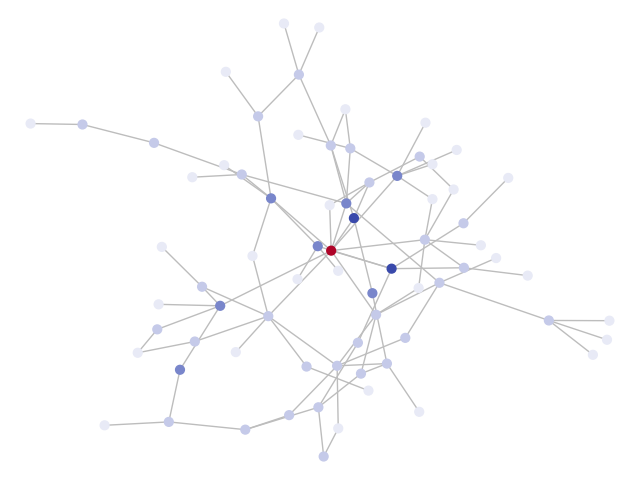
\includegraphics[width=0.7\linewidth]{basin-5-2}
    \caption{Exemple de bassin d'attraction pour une instance de taille 5 et une seule solution possible. Le bassin trouvé est de taille $70$ pour un espace de recherche de taille $5! = 120$. On peut ainsi en déduire la probabilité pour un joueur de se trouver dans ce bassin d'attraction.}
    \label{fig-basin}
\end{figure}
	}
	
\begin{definition}
    Un optimum local $x^*$ est une solution telle que toute solution voisine $x$ présente une fitness inférieure ou égale à celle de $x^*$.
    \begin{equation*}
        \forall x \in \mathcal{N}(x^*),~f(x) \leq f(x^*)
    \end{equation*}
\end{definition}

    \paragraph{Nombre d'optimums locaux (\texttt{nlo})}{
La modalité de l'espace de recherche donne une indication de la rugosité du paysage. Selon l'\Cref{obs-swap}, les joueurs peuvent exécuter des parcours adaptatif et cette mesure se révèle alors intéressante. Pour l'estimer plusieurs méthodes ont été considérées: échantillonnage aléatoire et échantillonnage via parcours adaptatifs. Dans la méthode proposée par \cite{alyahya}, des solutions candidates sont tirées uniformément aléatoirement et sont évaluées. On obtient ainsi une procédure de complexité $O(n \times |\mathcal{N}|)$ avec $n$ la taille de l'échantillon souhaité. La fiabilité de cet estimateur est largement dépendant de la taille choisie. Dans la méthode basée sur des parcours adaptatifs des solutions candidates sont choisies uniformément aléatoirement mais on procède à un parcours adaptatif dessus afin de trouver un optimum. Ce rapport n'étudie que des instances de taille n'excédant pas $7$ agents ce qui veut dire un maximum de $7! = 5040$ solutions possibles. Ce faible nombre permet de compter exhaustivement le nombre d'optimums locaux.
    }
	
	\paragraph{Auto-corrélation (\texttt{ac})}{Une autre mesure permettant l'estimation de la rugosité est l'auto-corrélation de la fonction fitness dans des parcours de l'espace de recherche. Si elle est haute alors la fitness ne varie pas beaucoup de voisin en voisin: le paysage est dit \textquote{plat}. On s'est intéressé dans ce projet à mesurer cette corrélation dans le voisinage des optimums. L'intuition est que si un optimum a un grand bassin d'attraction mais que la corrélation est grande, alors il sera difficile pour un joueur de naviguer jusqu'à l'optimum. On procède à des parcours aléatoires en partant d'optimums et la mesure \texttt{ac} est donnée par la formule suivante \cite{pitzer}
	\begin{equation*}
    \rho(n) = \frac{E\left[f(x_i) - \bar{f})(f(x_{i+n}) - \bar{f})\right]}{
        \sigma_f^2    
    }
	\end{equation*}
	avec $\sigma_f^2 = \bar{f^2} - \bar{f}^2$ la variance de fitness et $E$ la fonction d'espérance mathématique. On calcule ici $\rho(1)$ qui permet de calculer l'auto-corrélation le long du parcours.
	}
	
	\subsection{Apprentissage de la difficulté}
	
	Fort de ces mesures, il s'est agit ensuite d'établir la relation entre les caractéristiques d'une instance et la difficulté ressentie par les utilisateurs. Pour cela, l'application mobile (détaillée en~\Cref{app}) était très utile et il a été demandé à un grand nombre de personne de résoudre des instances. À chaque niveau résolu l'application enregistre les informations suivantes: le \textit{nombre de coups}, le \textit{temps de résolution} et une \textit{note de difficulté} donnée par le joueur. Un \textquote{coup} correspond à l'action de donner un objet à un agent. Les instances choisies pour ces collectes de données ainsi que leurs features sont visibles en~\Cref{tab-trainset}.
	
	Aucune corrélation directe entre les mesures développées dans ce projet et les difficultés reportées n'a pu être établie. Même la mesure simple de la taille du niveau n'est pas d'une grande aide (voir~\Cref{fig-size-diff}). Les notes sont distribuées quasiment également quelle que soit la taille des niveaux. Nous avons donc dû envisager des modèles de décision plus complexes.
	
	\begin{figure}[ht!]
	    \centering
	    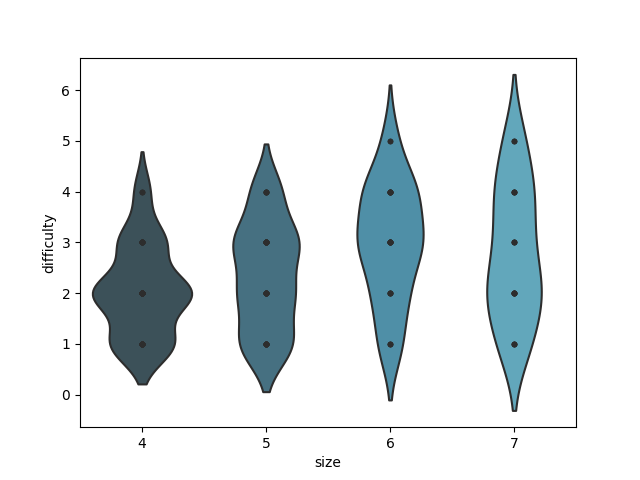
\includegraphics[width=0.7\linewidth]{size-diff-violin}
	    \caption{Difficulté en fonction de la taille}
	    \label{fig-size-diff}
	\end{figure}
	
	\subsubsection{Régression multiple, polynomiale et logistique}
	
	Disposant d'une expertise limitée dans le domaine de l'optimisation stochastique, nous avons d'abord opté pour une simple régression linéaire multiple permettant de prédire le niveau de difficulté d'une instance. On pourra donc utiliser toutes les mesures détaillées précédemment comme \textit{features} et tenter de prédire une des trois données récupérées des utilisateurs. Chacune cependant présente certains défauts: la difficulté ressentie semble être la plus intéressante pour définir la difficulté réelle d'un niveau mais est par définition subjective et sujette aux antécédents du joueur (formation, affinités mathématiques, etc). De plus, les joueurs gagnent de l'expérience à chaque instance résolue et leur ressenti en est impacté. Ceux qui commencent le jeu auront tendance à noter les premières instances jouées (souvent de moindre taille) hautes en difficulté et ceux plus experts noteront les dernières (de grande taille) moins difficiles. Il est difficile de savoir à quel point l'ordre dans lequel sont présentées les instances influe sur les ressentis. L'approche de ce projet demande des expériences plus poussées que ce qui a pu être fait.
	
	Le temps passé sur une instance également peut être facilement faussé si un joueur est dérangé pendant le jeu ou n'est tout simplement pas concentré dessus pendant toute la résolution. Enfin certains joueurs auront tendance à réfléchir mentalement uniquement et d'autres à utiliser abondamment le support à leur disposition, augmentant le nombre de coups. 
	
	Nous avons mis en place un ensemble d'apprentissage qui tente d'avoir le plus de diversité possible dans les features tout en évitant les instances à solution évidente. Une régression linéaire multiple a tout d'abord été testée sans grands espoirs (prédiction d'une valeur réelle à partir de plusieurs features) \cite{lr}. Dans ce premier modèle on dispose d'une matrice de features $X$ qui pour toute résolution reporte les caractéristiques de l'instance résolue. On dispose également d'un vecteur $Y$ qui pour chaque résolution associe la difficulté notée. Le but est de trouver la fonction la plus probable pour expliquer $Y$ à partir de $X$ et on utilise pour cela la méthode des moindres carrés. 
	
	On souhaite trouver un vecteur de poids $w$ de façon à ce que $\hat{Y} = wX + b$ soit le plus proche possible de $Y$. Pour cela l'erreur $E$ de l'\Cref{eq-error} est minimisée; Le \textquote{bias term} est inclu dans $w$ et une colonne de $1$ est ajoutée aux features de $X$.
\begin{equation}
\label{eq-error}
E = \sum_i (y_i - w^Tx_i)^2
\end{equation}
Mettre les erreurs \textit{au carré} nous permet de dériver l'erreur par rapport à toutes les composantes de $w$ et de chercher les valeurs pour lesquelles ces dérivées s'annulent. On peut écrire l'erreur sous forme matricielle (\Cref{eq-mat}).
\begin{align}
E &= \sum_i (y_i - w^Tx_i)^2 \nonumber\\
E &= (Y - Xw)^T(Y - Xw) \nonumber\\
E &= Y^TY - Y^TXw - (Xw)^TY + (Xw)^T(Xw) \nonumber\\
E &= Y^TY - Y^TXw - w^Tx^TY + w^TX^TXw \label{eq-mat}
\end{align}
On peut alors calculer la dérivée partielle par rapport à $w$ (grâce à \cite{petersen}).
\begin{equation*}
\frac{\partial{E}}{\partial{w}} = -2X^TY + 2X^TXw
\end{equation*}
Chercher $w$ tel que cette dérivée s'annule revient alors à résoudre l'équation suivante.
\begin{align*}
\frac{\partial{E}}{\partial{w}} = 0 &\rightarrow X^TXw = X^TY \\
&\rightarrow w = (X^TX)^{-1}X^TY
\end{align*}

Les calculs sont délégués à la librairie \texttt{sklearn} et le modèle \texttt{LinearRegression} est utilisé sur l'ensemble des données. À la date d'écriture de ce rapport cet ensemble comprend $182$ exemples et $13$ features différentes. Il est partagé en ensemble d'apprentissage et ensemble de test dans les proportions 80\%/20\% aléatoirement. Pour mesurer la fiabilité du modèle la mesure $r^2$ est utilisée, définie comme suit.
\begin{equation*}
    r^2 = 1 - \frac{E}{\sum_i (y_i - \bar{y})^2}
\end{equation*}
On l'interprète comme une mesure d'erreur du modèle par rapport à la prédiction de la moyenne. Un $r^2$ de $1$ indique un modèle sans erreur, un $r^2$ à $0$ indique un modèle qui ne prédit pas mieux que la moyenne. Un $r^2$ inférieur à $0$ veut généralement dire un modèle mauvais car prédisant moins bien que la moyenne. 

Dans notre projet, le meilleur score trouvé est de $0.25$ pour une erreur carrée moyenne (MSE) de $0.84$. Étant donnée le faible nombre d'exemples ce score est grandement impacté par la répartition dans les ensembles d'apprentissage et de test. Néanmoins, tester d'autres modèles nous semblait important et l'étape logique suivante était un apprentissage via régression polynomiale. Pour cela on augmente artificiellement la dimensionnalité des features en ajoutant des termes dans la matrice $X$. Ils correspondent aux features existantes avec un degré supérieur. Ainsi notre modèle précédent $y = w_0x_0 + w_1x_1 + ... + w_nx_n$ se trouve transformé en $y = w_0x_0 + w_1x_1 + w_2x_2 + w_{11}x_1^2 + w_{22}x_2^2 + w_{12}x_1x_2$ pour un modèle à deux features et un degré maximal de $2$ (\cite{sinha}). Puisque le passage à un modèle polynomial peut entraîner des poids élevés dans $w$ dans les domaines où il n'existe pas beaucoup de donnée, une régularisation de type Ridge est utilisée (\Cref{eq-ridge}).
\begin{equation}
\label{eq-ridge}
E_{RIDGE} = \sum_i (y_i - \hat{y}_i)^2 + \alpha|w|^2
\end{equation}
On pénalise les grands poids en ajoutant leur magnitude (norme L2 de $w$) au carré au coût. Cela permet de réduire les risques de sur-apprentissage. Malgré ces changements malheureusement, même en montant jusqu'à un degré $5$ on obtient un $r^2$ de $0.30$ et une MSE de $0.79$. Au vu de ces résultats peu intéressants, une dernier type de régression a été testé.

Dans la régression logistique il n'est plus question de prédire une valeur réelle mais un entier qui correspond à la classe de difficulté. Dans l'application les joueurs peuvent la noter en choisissant une valeur entre $1$ et $5$ et c'est cette valeur qui servira donc de classe dans ce modèle. Par manque de temps les calculs sous-jacents n'ont pas été étudiés et le modèle a été testé directement en s'inspirant des exemples trouvés dans la documentation de \texttt{sklearn}. Ce modèle est par ailleurs un classifier et on calcule donc son score comme le pourcentage de bonne réponses. D'après nos tests, le plus haut score que nous puissions obtenir est de $0.48$ pour une MSE de $1.08$.

\subsubsection{Arbres de décision}

La dernière approche abordée a été de faire appel aux classifiers arbres de décision souvent abordés dans notre formation \cite{dt}. L'idée y est de construire un arbre dont les feuilles correspondent aux classes à prédire. Chaque nœud correspond ensuite à une décision concernant une des features. Lorsque les nœuds sont construits, l'algorithme d'apprentissage tente de trouver les features et valeurs associées promettant le plus de discrimination au sein des exemples (l'entropie de Shannon est souvent utilisée). On utilise ici aussi la librairie \texttt{sklearn} pour produire l'arbre.

Les premières constructions montrent des scores élevées mais après plus proche examination semblent ne pas pouvoir se généraliser convenablement. En effet, la plupart des feuilles ne concernent que quelques exemples (un ou deux) et l'arbre est généralement très profond. On en déduit un sur-apprentissage et un nombre minimal d'exemples par feuille est posé à 10\% de l'ensemble d'apprentissage. Malheureusement le score trouvé est alors seulement de $0.40$ au mieux (l'arbre correspondant est visible en~\Cref{tree}). Il serait peut être bon d'explorer les forêts aléatoires.

\end{document}